\documentclass{cmc}
\usepackage{makecell}
\begin{document}

\pagestyle{fancy}
\lhead{\textit{\textbf{Computational Motor Control, Spring 2020} \\
    Webots exercise, Lab 7, GRADED}} \rhead{Student \\ Names}

\section*{Student names: \ldots (please update)}


\section*{Swimming with Salamandra robotica – CPG Model}
\label{sec:exploring-swimming}

In this project you will control a salamander-like robot Salamandra
robotica II for which you will use Python and the PyBullet physics
engine. Now you have an opportunity to use what you’ve learned until
now to make the robot swim and eventually walk. In order to do this,
you should implement a CPG based swimming controller, similarly to the
architecture shown in Figure~\ref{fig:controller-model}.

The project is based on the research of \cite{Crespi2013},
\cite{Karakasiliotis2013} and \cite{ijspeert2007swimming}. It is strongly
recommended to review \cite{ijspeert2007swimming} and its supplementary material
provided on the Moodle. You will be tasked with replicating and
studying the Central Pattern Generator (CPG).

\corr{\textit{NOTE : }} The session this week will be an introduction to the
final project. You will be installing the PyBullet physics engine will and get
to familiarise with it. You will start implementing the CPG network which will
eventually control the robot.

\begin{figure}[h]
  \centering
  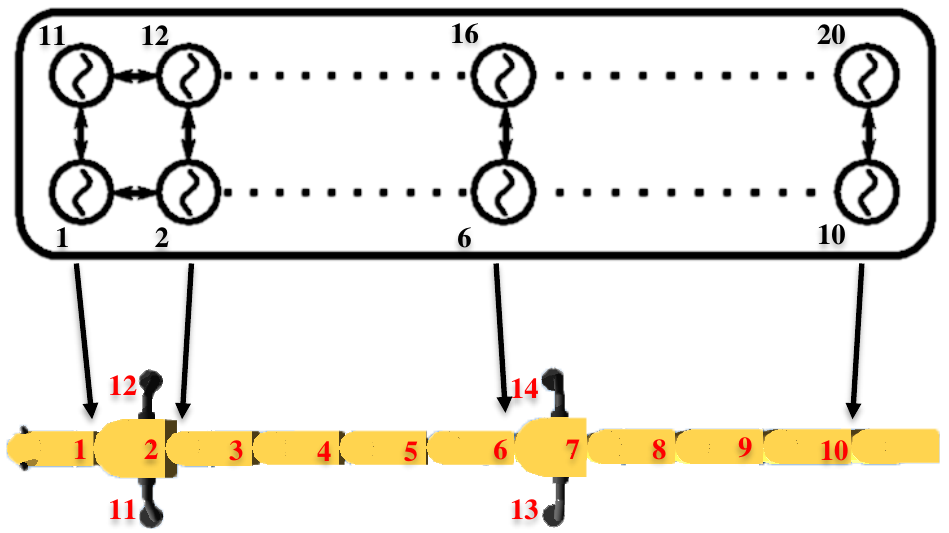
\includegraphics[width=0.5\textwidth]{figures/model_controller.png}
  \caption[Controller model]{A double chain of oscillators controlling
    the robot’s spine.}
  \label{fig:controller-model}
\end{figure}

\begin{figure}[ht]
  \centering 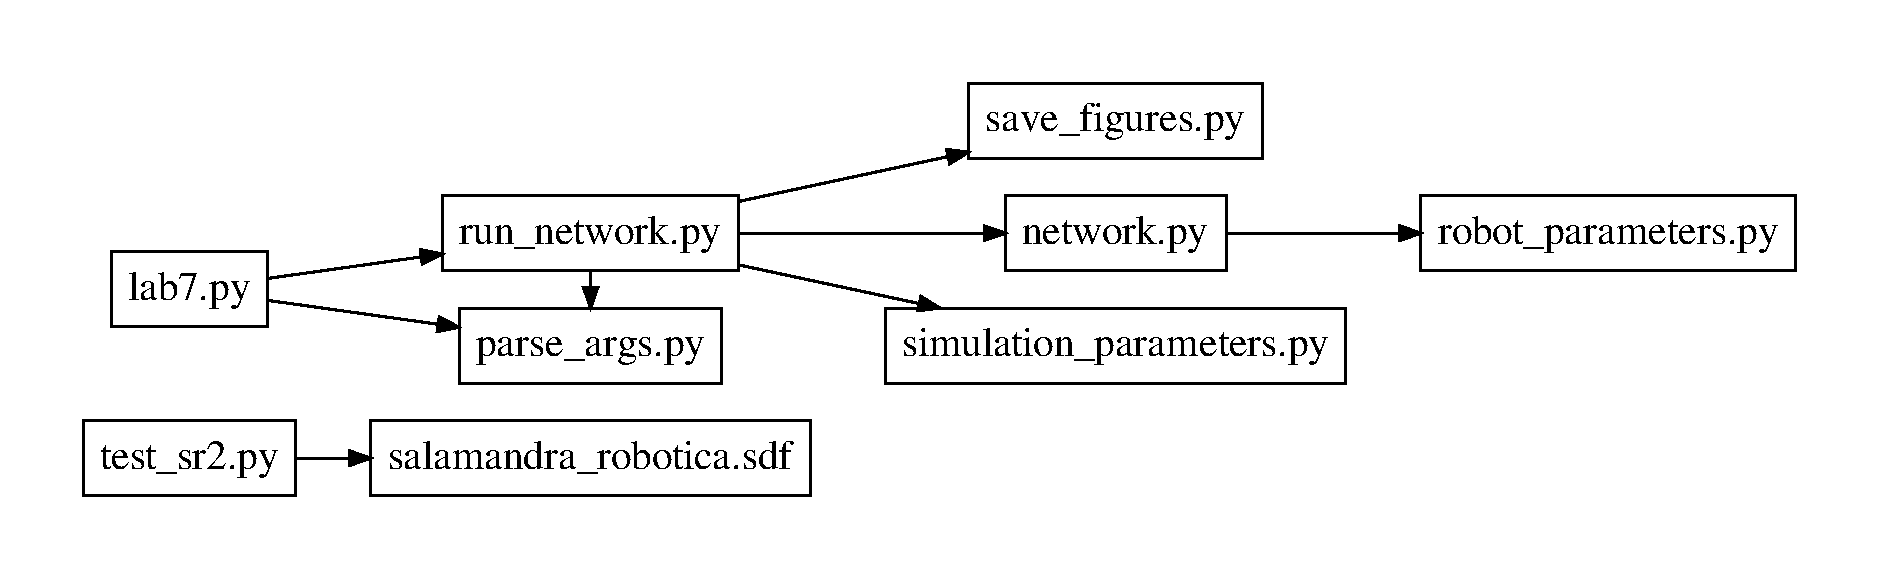
\includegraphics[width=1.0\textwidth]{figures/files}
  \caption{\label{fig:files} Exercise files dependencies. In this lab, you will
    be modifying \fileref{run\_network.py}, \fileref{network.py},
    \fileref{robot\_parameters.py} and \fileref{simulation\_parameters.py}}
\end{figure}

% \newpage

\subsection*{Code organization}
\label{subsec:code}

\begin{itemize}
\item \corr{\textbf{test\_sr2.py}} - This is a file to verify that Pybullet was
  installed correctly. It is important to make sure that this file works as it
  will be necessary for the project.
\item \corr{\textbf{network.py}} - This
  file contains the different classes and functions for the CPG network and the
  Ordinary Differential Equations (ODEs). You can implement the network
  parameters and the ODEs here. Note that some parameters can be obtained from
  pythonController.py to help you control the values.
\item
  \corr{\textbf{robot\_parameters.py}} -
  This file contains the different classes and functions for the parameters of
  the robot, including the CPG network parameters. You can implement the network
  parameters here. Note that some parameters can be obtained from
  SimulationParameters class in \corr{simulation\_parameters.py} and sent by
  \corr{exercise\_\#.py} to help you control the values (refer to example).
\item
  \corr{\textbf{simulation\_parameters.py}}
  - This file contains the SimulationParameters class and is provided for
  convenience to send parameters to the setup of the network parameters in
  \corr{robot}\-\corr{\_parameters.py}. All the values provided in SimulationParameters
  are actually logged in \corr{cmc}\-\corr{\_robot.py}, so you can also reload these
  parameters when analyzing the results of a simulation.
\item \corr{\textbf{run\_network.py}} -
  By running the script from Python, PyBullet will be bypassed and you will run
  the network without a physics simulation. Make sure to use this file for
  question 7a to help you with setting up the CPG network equations and
  parameters and to analyze its behavior. This is useful for debugging purposes
  and rapid controller development since starting the Webots simulation with
  physics takes more time.
\item \corr{\textbf{parse\_args.py}} -
  Used to parse command line arguments for run\_network.py and plot\_results.py
  and determine if plots should be shown or saved directly. \textit{You do not
    need to modify this files.}
\item \corr{\textbf{save\_figures.py}} -
  Contains the functions to automatically detect and save figures. \textit{You
    do not need to modify this files.}
\end{itemize}

% \newpage

\section*{Prerequisites}

Make sure you have successfully installed Pybullet by following the instructions
outlined in \corr{\textbf{pybullet\_introduction.pdf}}. The script
\corr{\textbf{test\_sr2.py}} will allow you to verify by loading and visualising
the robot. Please refer to the TAs if you face any issue with running this file.


\newpage

\section*{Questions}

The exercises are organized such that you will have to first implement the
oscillator network model in \corr{run\_network.py} code and analyze it before
connecting it to the body in the physics simulation.  Exercise 7a describes the
questions needed to implement the oscillator models. After completing exercise
7a you should have an oscillator network including both the spinal CPG and limb
CPG.

The remainder of the exercises will be distributed next week.


\subsection*{7a. Implement a double chain of oscillators along with
  limb CPG's}
\label{sec:implement-chain}

Salamandra robotica has 10 joints along its spine and 1 joint for each
limb. The controller is defined as

\begin{equation}
  \label{eq:dphase}
  \dot{\theta}_i = 2 \pi f + \sum_j r_j w_{ij} sin(\theta_j - \theta_i - \phi_{ij})
\end{equation}

\begin{equation}
  \label{eq:dr}
  \dot{r}_i = a (R_i - r_i)
\end{equation}

\begin{equation}
  \label{eq:output}
  q_i = r_i(1 + cos(\theta_i)) - r_{i+10}(1 + cos(\theta_{i+10})) \text{ if body joint}
\end{equation}

with $ \theta_i $ the oscillator phase, f the frequency, $ w_{ij} $ the coupling
weights, $ \phi_{ij} $ the nominal phase lag (phase bias), $ r_i $ the
oscillator amplitude, $ R_i $ the nominal amplitude, $ a $ the convergence
factor and $ q_i $ the spinal joint angles. For more information, please refer
to \cite{ijspeert2007swimming}. Also note how these are the same equations,
although Equation \eqref{eq:dr} has been simplified into a first order ODE in
order to simplify the implementation in this project.


\begin{enumerate}
\item Implement the double chain oscillator model using the functions
  \fileref{network.py::network\_ode}. Test your implementation by running the
  network using \fileref{run\_network.py}. For the network parameters check
  lecture slides (pay attention to different number of segments). You can also
  find more information in \cite{ijspeert2007swimming} (especially in the
  supplementary material). You can set all the network parameters in the
  \fileref{robot\_parameters.py::RobotParameters}. To facilitate your work, you
  could start by only implementing the network for the body oscillators
  ($i=[0, ..., 19]$) and ignoring the leg oscillators ($i=[20, ..., 23]$). Refer
  to \corr{network::RobotState} and
  \corr{robot\_parameters.py::}\-\corr{RobotParameters} for the dimensions of
  the state and the network parameters respectively.

\item Implement the output of your CPG network to generate the spinal joint
  angles according to equation \ref{eq:output}. Implement this in the function
  \fileref{network.py::motor\_output}. Verify your implementation in by running
  the Python file \fileref{run\_network.py}.


\item Implement a drive and show that your network can generate swimming and
  walking patterns similarly to \cite{ijspeert2007swimming}. Try to reproduce
  the plots in \ref{fig:science_oscillator_patterns} and
  \ref{fig:science_oscillator_properties}


  \textbf{Hint:} The state for the network ODE is of size 48 where the first 24
  elements correspond to the oscillator phases $\theta_i$ of the oscillators and
  the last 24 elements correspond to the amplitude $r_i$. The initial state is
  set in the init of \corr{network.py::SalamanderNetwork}.
\end{enumerate}

\begin{figure}[H]
  \centering
  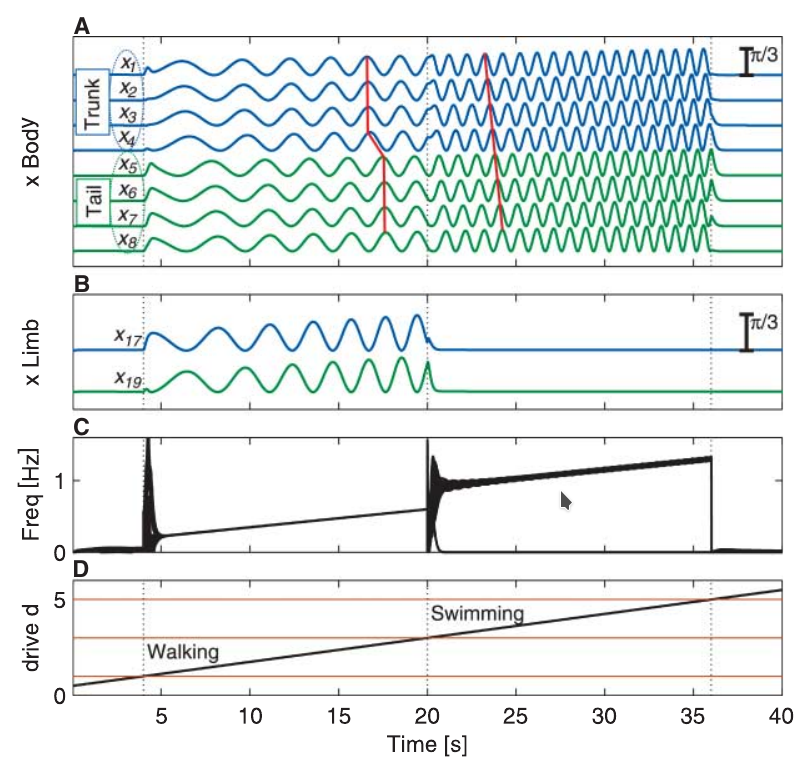
\includegraphics[width=0.7\textwidth]{figures/science_oscillator_patterns}
  \caption{Oscillator patterns from \cite{ijspeert2007swimming}, see
    \cite{ijspeert2007swimming} for details}
  \label{fig:science_oscillator_patterns}
\end{figure}

\begin{figure}[H]
  \centering
  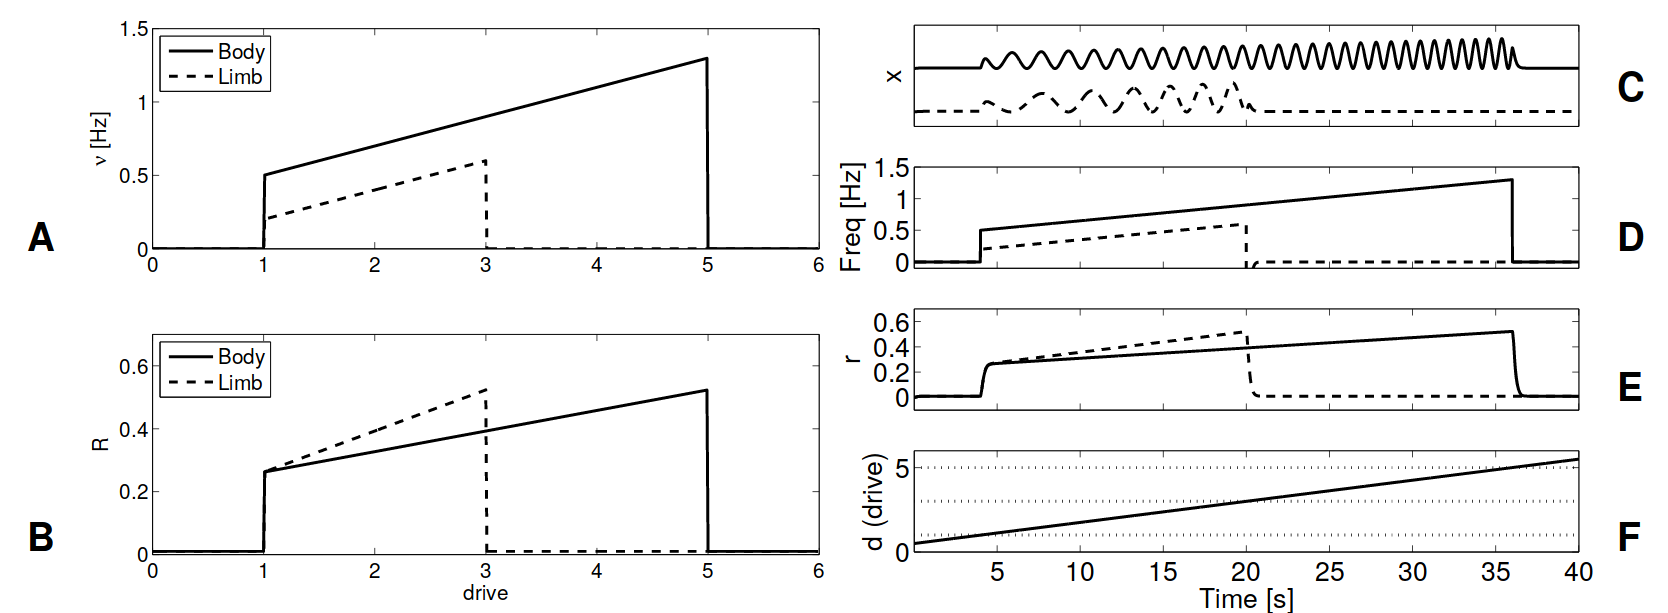
\includegraphics[width=1.0\textwidth]{figures/science_oscillator_properties}
  \caption{Oscillator properties from \cite{ijspeert2007swimming} supplementary
    material, see \cite{ijspeert2007swimming} for details}
  \label{fig:science_oscillator_properties}
\end{figure}



\newpage

\bibliography{lab7}
\label{sec:references}
\bibliographystyle{ieeetr}


% \newpage

% \section*{APPENDIX}
% \label{sec:appendix}

\end{document}

%%% Local Variables:
%%% mode: latex
%%% TeX-master: t
%%% End: